\section{Methodology}

\begin{figure}[h!]
  \centering 
    \includegraphics[width=0.98\linewidth]{figs/overview}
  \caption{Overview of the proposed 3D anomaly detection framework. From left to right: input point cloud; hierarchical patch tokens produced by a frozen, pretrained point cloud Transformer; tokens reordered by the geometric semantic-aware sorter (GSAS) into a surface-aware, semantically coherent sequence; a selective state-space adapter (Mamba / S6) that fuses ordered tokens into context-enhanced slot features; a sparse Anomalous Feature Generator (training only) that injects feature-space perturbations to supervise a compact cross-patch attention discriminator; discriminator logits are reprojected to the point cloud to produce a per-point anomaly heatmap and a global point cloud score.}
  \label{fig:overview}
\end{figure}

We address efficient 3D anomaly detection that requires minimal task-specific training while preserving geometric structure and long-range contextual reasoning. As illustrated in Figure \ref{fig:overview}, given an input point cloud \(\mathcal{P} = \{\mathbf{p}_i \in \mathbb{R}^3\}_{i=1}^N\), the proposed pipeline leverages a frozen pre-trained point cloud Transformer together with a compact set of lightweight adapters to generate spatially coherent and anomaly-sensitive representations. The backbone consists of \(L\) encoder layers, each producing \(M\) patch tokens of dimension \(D\); we denote the patch-token matrix and class token at layer \(i\) as \(\mathbf{T}_i \in \mathbb{R}^{M\times D}\) and \(c_i \in \mathbb{R}^{1\times D}\), respectively, and collect the hierarchical token set \(\mathbf{T} = \{\mathbf{T}_1, \dots, \mathbf{T}_L\}\) with a total of \(T = L \cdot M\) tokens. These unordered layer-wise tokens are transformed into a semantically ordered sequence \(\mathbf{T}_{\mathrm{ord}} \in \mathbb{R}^{T\times D}\), subsequently fused into enriched contextual features \(y_{1:T} \in \mathbb{R}^{T\times D}\), and finally scored by a lightweight attention-based discriminator for per-patch anomaly localization. The geometric semantic-aware sorter (GSAS) establishes a differentiable soft-permutation that orders the hierarchical tokens while preserving geometric locality and semantic consistency. The Mamba adapter, a linear-time state-space model, efficiently fuses the ordered sequence to yield context-enhanced features \(y_{1:T}\) that retain both local fidelity and global awareness. A selective anomaly generator operates during training to inject sparse feature-space perturbations, enabling effective supervision without real defect labels. The cross-patch discriminator then aggregates contextual cues through a compact attention mechanism to output patch-level anomaly logits, which are reprojected to points for precise localization. 

\subsection{Backbone}

Given an input point cloud \(\mathcal{P} = \{\mathbf{p}_i\in\mathbb{R}^3\}_{i=1}^N\), the backbone produces local patch embeddings and a hierarchical set of Transformer tokens that preserve patch identities across layers. We apply Farthest Point Sampling (FPS) to select \(M\) patch centers \(\{p_j\in\mathbb{R}^3\}_{j=1}^M\), where index \(j\) denotes a patch center, and for each center we collect a fixed-size neighborhood of \(K\) points via \(K\)-nearest neighbors (KNN). Each neighborhood is embedded by a lightweight PointNet encoder followed by a positional-encoding MLP to yield an initial patch embedding \(x_j^{(0)}\in\mathbb{R}^D\), for \(j=1,\dots,M\). The \(M\) initial embeddings are concatenated with a global class token \(c_0\in\mathbb{R}^{1\times D}\) to form the Transformer input \([c_0;\mathbf{T}_0]\), where \(\mathbf{T}_0=[x_1^{(0)};\dots;x_M^{(0)}]\in\mathbb{R}^{M\times D}\). These are passed to the frozen Point-MAE Transformer pretrained on ShapeNet~\cite{pang2022masked,chang2015shapenet}. Formally, the \(i\)-th Transformer block \(\ell_i(\cdot)\) computes
\begin{equation}
[c_i;\,\mathbf{T}_i] \;=\; \ell_i([c_{i-1};\,\mathbf{T}_{i-1}]), \qquad i=1,\dots,L,
\end{equation}
with \(\mathbf{T}_i=[t_{i,1};\dots;t_{i,M}]\in\mathbb{R}^{M\times D}\) and \(c_i\in\mathbb{R}^{1\times D}\). The spatial coordinates \(\{p_j\}\) remain associated with their patch index \(j\) and are reused at every Transformer layer; consequently token \(t_{i,j}\) at layer \(i\) corresponds to the same geometric patch center \(p_j\). The backbone therefore outputs the initial patch embeddings \(\{x_j^{(0)}\}_{j=1}^M\) with \(x_j^{(0)}\in\mathbb{R}^D\), the hierarchical tokens \(\{\mathbf{T}_i\}_{i=1}^L\) with \(\mathbf{T}_i\in\mathbb{R}^{M\times D}\), the sequence of class tokens \(\{c_i\}_{i=1}^L\) with \(c_i\in\mathbb{R}^{1\times D}\), and the retained patch centers \(\{p_j\}_{j=1}^M\in\mathbb{R}^3\). Optionally, these tokens may be viewed as a flattened set \(\mathbf{T}=\{\mathbf{T}_1,\dots,\mathbf{T}_L\}\) of \(T=L\cdot M\) tokens in \(\mathbb{R}^{T\times D}\).

\subsection{Geometric Semantic-Aware Sorter (GSAS)}
\label{sec:gsas}

\begin{figure}[h!]
  \centering 
    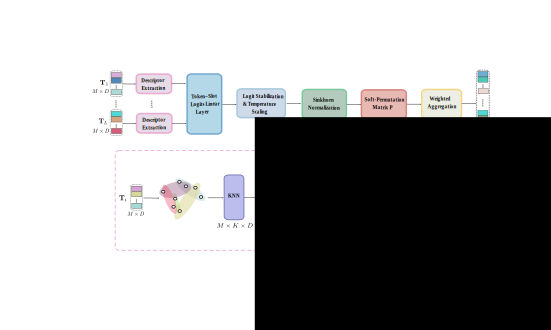
\includegraphics[width=0.98\linewidth]{figs/GSAS}
  \caption{Overview of geometric semantic-aware sorter (GSAS).}
  \label{fig:GSAS}
\end{figure}

Given input tokens \(X\in\mathbb{R}^{T\times D}\), where \(X\) denotes the flattened collection of all per-layer tokens \(t_{i,j}\) produced by the backbone (so that each \(\mathbf{T}_i=[t_{i,1};\dots;t_{i,M}]\in\mathbb{R}^{M\times D}\) and \(T=L\cdot M\)), and given the unique patch centers \(\{p_j\in\mathbb{R}^3\}_{j=1}^M\), GSAS produces a differentiable ordering of the \(T\) tokens that preserves local surface adjacency and semantic affinity. As illustrated in Figure ~\ref{fig:GSAS}, we first summarizes local geometry and same-layer semantics, then computes token-slot affinities, converts affinities to an approximately doubly-stochastic assignment, and finally aggregates tokens into ordered slots for downstream fusion.

We construct a kNN graph on the unique patch centers and denotes the neighbor set of patch \(j\) by \(\mathcal{N}_{\mathrm{patch}}(j)\subset\{1,\dots,M\}\). For a token \(t\) corresponding to \((i,j)\) with \(i=i(t)\) and \(j=j(t)\), GSAS computes a permutation-invariant local descriptor by aggregating features from the same Transformer layer \(i\) of neighboring patches:
\begin{equation}
u_{i,j} \;=\; \mathrm{MaxPool}\Big(\big\{\,W_{\downarrow}\,t_{i,u} + b_{\downarrow} \ \big|\ u\in\mathcal{N}_{\mathrm{patch}}(j)\big\}\Big)\in\mathbb{R}^{d_a},
\end{equation}
where \(W_{\downarrow}\in\mathbb{R}^{d_a\times D}\) and \(b_{\downarrow}\in\mathbb{R}^{d_a}\). The module collects these descriptors into \(E\in\mathbb{R}^{T\times d_a}\) by setting \(E_{t,:}=u_{i(t),j(t)}\). The descriptor \(E\) summarizes local geometry while preserving layer-specific semantics, and GSAS uses \(E\) to inform the affinity computation in the next step. We compute raw token-slot affinities from the descriptors:
\begin{equation}
\mathbf{G} \;=\; E\,W_{\uparrow} + \mathbf{1}\,b_{\uparrow}^\top \in\mathbb{R}^{T\times T},
\end{equation}
with \(W_{\uparrow}\in\mathbb{R}^{d_a\times T}\), \(b_{\uparrow}\in\mathbb{R}^T\), and \(\mathbf{1}\in\mathbb{R}^{T\times 1}\). The matrix \(\mathbf{G}\) encodes unnormalized affinities between tokens and ordered slots, and GSAS processes \(\mathbf{G}\) to produce a differentiable assignment that can be optimized end-to-end.

For numerical stability we subtract the column-wise maximum \(v\in\mathbb{R}^T\) with entries \(v_s=\max_t \mathbf{G}_{t,s}\), applies temperature scaling and exponentiation, and normalizes with the Sinkhorn operator:
\begin{equation}
\tilde{\mathbf{G}} \;=\; (\mathbf{G} - \mathbf{1}\,v^\top)/\tau,
\end{equation}
\begin{equation}
P \;=\; \mathrm{Sinkhorn}\big(\exp(\tilde{\mathbf{G}}),\,K_{\mathrm{sink}}\big)\in[0,1]^{T\times T},
\end{equation}
where \(\tau>0\) denotes the temperature and \(K_{\mathrm{sink}}\) the number of iterations. The soft-permutation \(P\) is approximately doubly-stochastic and differentiable, and GSAS uses \(P\) to aggregate token features into a semantically coherent ordered sequence. We aggregate tokens into ordered slots by weighted summation:
\begin{equation}
\mathbf{T}_{\mathrm{ord}} \;=\; P^\top X \in\mathbb{R}^{T\times D},
\end{equation}
\begin{equation}
\mathbf{T}_{\mathrm{ord}}[s,:]=\sum_{t=1}^T P_{t,s}\,X_t.
\end{equation}
The aggregation yields one feature vector per ordered slot while preserving differentiability so that gradients propagate to \(W_{\downarrow},b_{\downarrow},W_{\uparrow},b_{\uparrow}\). The ordered tokens \( \mathbf{T}_{\mathrm{ord}}\) therefore provide the contiguous, semantically coherent input required by the subsequent fusion module.

We include two auxiliary regularizers to prevent degenerate assignments and to encourage geometric locality. The column-wise entropy penalty discourages diffuse assignments into a given slot:
\begin{equation}
\mathcal{L}_{\mathrm{ent}} \;=\; \frac{1}{T}\sum_{s=1}^T H(P_{:,s}),\qquad
H(\pi)=-\sum_{t}\pi_t\log(\pi_t+\epsilon_{\mathrm{ent}}),
\end{equation}
with \(\epsilon_{\mathrm{ent}}>0\) for numerical stability. The entropy penalty directly biases the columns of \(P\) toward concentrated assignments and thus improves the quality of aggregation in Eq. for \(\mathbf{T}_{\mathrm{ord}}\). The locality penalty measures expected slot positions \(\mu_t\) and biases them to align with geometric affinities:
\begin{equation}
\mu_t \;=\; \sum_{s=1}^T \tilde s\,P_{t,s}\in[0,1],
\end{equation}
\begin{equation}
w_{t,u} \;=\; \exp\!\big(-\|p_{j(t)}-p_{j(u)}\|^2/\sigma_p^2\big),
\end{equation}
\begin{equation}
\mathcal{L}_{\mathrm{loc}} \;=\; \sum_{t=1}^T \frac{1}{\sum_{u=1}^T w_{t,u} + \epsilon_{\mathrm{norm}}}\sum_{u=1}^T w_{t,u}\,\big(\mu_t - \mu_u\big)^2,
\end{equation}
where \(\tilde s=(s-1)/\max(1,T-1)\), \(\sigma_p\) is a bandwidth parameter, and \(\epsilon_{\mathrm{norm}}>0\) stabilizes the normalization. The locality penalty directly influences \(\mu_t\) and thus biases the soft-permutation \(P\) to place geometrically adjacent tokens into nearby slots.

\subsubsection{Mamba Feature Adapter}

Given the GSAS-ordered slot tokens \(\mathbf{T}_{\mathrm{ord}}\in\mathbb{R}^{T\times D}\) we denote the row-wise sequence by
\begin{equation}
x_{1:T},\qquad x_t=\mathbf{T}_{\mathrm{ord}}[t,:]\in\mathbb{R}^D,\quad t=1,\dots,T.
\end{equation}
We integrate this sequence with a selective state-space adapter from the S6/Mamba family \cite{gu2023mamba}. The adapter conditions its discrete dynamics on the current token, allowing per-token adjustment of the effective temporal scale and input coupling while preserving linear-time complexity. The selective discrete recurrence may be written compactly as
\begin{equation}
h_t = A_t\,h_{t-1} + B_t\,x_t,\qquad h_0=\mathbf{0}\in\mathbb{R}^S,
\end{equation}
where \(h_t\in\mathbb{R}^S\) is the SSM hidden state at step \(t\) and \((A_t,B_t)\) are token-conditioned discrete matrices obtained from continuous-time proposals via the S6 discretization \cite{gu2023mamba}. The S6 output projection produces an adapted slot feature by combining the recurrent state with a residual path from the input:
\begin{equation}
\tilde{q}_t = C_t\,h_t + D\,x_t \in\mathbb{R}^D,
\end{equation}
where \(C_t\) is token-conditioned and \(D\in\mathbb{R}^{D\times D}\) is a learned residual projection that preserves per-token fidelity. To stabilize training and allow the model to adaptively gate the SSM contribution we apply a lightweight gating and normalization:
\begin{equation}
q_t = \mathrm{LayerNorm}\!\Big( x_t + \sigma\big(g(x_t)\big)\odot \tilde{q}_t \Big),
\end{equation}
where \(g:\mathbb{R}^D\!\to\!\mathbb{R}^D\) is a small projection, \(\sigma\) is the sigmoid, and \(\odot\) denotes elementwise multiplication. Finally, the context-enriched token sequence is assembled as
\begin{equation}
Q = [q_1,\dots,q_T]^\top \in \mathbb{R}^{T\times D},
\end{equation}
which is passed to the downstream discriminator and heads for anomaly scoring. 

\subsection{Anomalous Feature Generator}

Given adapted tokens \(Q\in\mathbb{R}^{T\times D}\) produced by the Mamba adapter, where the rows are \(q_t\in\mathbb{R}^D\) for \(t=1,\dots,T\), the anomalous feature generator synthesizes sparse, feature-space perturbations to emulate localized defects during training. We generate a binary corruption mask, samples isotropic Gaussian perturbations in token space, and combines these quantities to produce corrupted tokens \(\tilde{q}_t\) that serve as positive supervision for the discriminator. The module samples an independent Bernoulli mask per slot:
\begin{equation}
m_t \sim \mathrm{Bernoulli}(p),\qquad m_t\in\{0,1\},
\end{equation}
with \(p\in(0,1)\) controlling expected corruption sparsity. The mask \(m_t\) determines which slots receive perturbations; consequently the mask provides binary supervisory labels for corrupted versus clean slots during training and guides the subsequent noise injection. We sample additive isotropic Gaussian noise in the canonical token space:
\begin{equation}
\varepsilon_t \sim \mathcal{N}\big(0,\sigma^2 I_D\big),
\end{equation}
with scale parameter \(\sigma>0\). The noise \(\varepsilon_t\) provides a generic, directionally unbiased perturbation in feature space; consequently the module uses this noise, when selected by \(m_t\), to produce pseudo-anomalous embeddings that remain in the same representational space as the adapted tokens \(q_t\). The module forms the pseudo-anomalous token by combining the adapted token, the mask, and a learnable rescaling:
\begin{equation}
\tilde{q}_t \;=\; q_t + \gamma\, m_t\, \varepsilon_t,
\end{equation}
where \(\gamma\ge 0\) denotes a learnable scalar that rescales the injected perturbation. The factor \(\gamma\) enables the model to adapt the effective perturbation magnitude during training; consequently the corrupted token \(\tilde{q}_t\) preserves the original feature \(q_t\) when \(m_t=0\) and expresses a controlled deviation when \(m_t=1\). The generator is active only during training; at inference time the mask is fixed to \(m_t\equiv 0\) and all tokens remain uncorrupted.

The design choice to inject sparse feature-space perturbations targets realistic industrial defects that are spatially localized and semantically subtle. The descriptor and fusion stages output context-enriched features \(q_t\) that already encode geometric and semantic information; therefore perturbing \(q_t\) in feature space produces anomalies that challenge the discriminator while avoiding unrealistic point-level artifacts. A global noise alternative would not preserve a normal manifold for the majority of slots and would reduce the signal-to-noise ratio for localization, and a per-layer independent corruption would not emulate cross-layer contextual inconsistencies that the discriminator must detect; consequently selective feature-space corruption provides a stronger and more realistic supervisory signal for per-slot anomaly localization. Because sparse corruption can induce class imbalance between corrupted and clean slots, we validate \(p\) on held-out data and mitigate imbalance via weighted loss or controlled sampling as described in the training procedure. The mask vector and corrupted tokens are therefore used directly as training inputs and labels for the cross-patch discriminator. The input to the anomalous feature generator is \(Q\in\mathbb{R}^{T\times D}\) (rows \(q_t\in\mathbb{R}^D\)) and the primary outputs are the corrupted token matrix \(\tilde{Q}=[\tilde{q}_1,\dots,\tilde{q}_T]^\top\in\mathbb{R}^{T\times D}\) and the binary mask \(m\in\{0,1\}^T\). The corrupted tokens \(\tilde{Q}\) and mask \(m\) are then consumed by the cross-patch discriminator for supervised anomaly learning during training; at inference the generator is disabled and \(\tilde{Q}=Q\).

\subsection{Cross-Patch Attention Discriminator}

Given corrupted tokens \(\tilde{Q}\in\mathbb{R}^{T\times D}\) and binary mask \(m\in\{0,1\}^T\) produced by the anomalous feature generator (training) or given clean tokens \(Q\in\mathbb{R}^{T\times D}\) at inference, and given patch centers \(\{p_t\in\mathbb{R}^3\}_{t=1}^T\), the discriminator produces contextualized per-slot logits \(s_t\in\mathbb{R}\) for \(t=1,\dots,T\). The discriminator jointly processes all slots to enable context-aware anomaly scoring that leverages spatial positional information derived from patch centers. The module computes positional embeddings from patch centers:
\begin{equation}
e_t \;=\; \mathrm{PE\text{-}MLP}(p_t) \in\mathbb{R}^D.
\end{equation}
The positional embedding \(e_t\) provides explicit spatial context and the module uses \(e_t\) to augment token features before attention. We form the discriminator input by combining corrupted or clean tokens with positional embeddings:
\begin{equation}
\hat{q}_t \;=\; \big(m_t\,\tilde{q}_t + (1-m_t)\,q_t\big) + e_t \;=\; q_t + m_t(\gamma\varepsilon_t) + e_t.
\end{equation}
The input \(\hat{q}_t\) therefore contains the appropriate training-time corruption when \(m_t=1\) and otherwise equals the clean token plus spatial embedding; the module uses \(\hat{q}_{1:T}\) as input to the attention layer.

The discriminator applies a single multi-head self-attention layer to jointly contextualize all slot inputs. The module denotes the number of heads by \(H\) and the per-head dimension by \(d_{\mathrm{head}}=D/H\). The module computes the contextualized features
\begin{equation}
Z \;=\; \mathrm{MHA}(\{\hat{q}_t\}_{t=1}^T) \in\mathbb{R}^{T\times D}.
\end{equation}
The multi-head attention mixes information across slots so that each row \(Z_t\) encodes both local evidence and global context; the module then uses \(Z\) to produce per-slot anomaly scores. We map contextualized features to scalar logits via a shared MLP head:
\begin{equation}
s_t \;=\; \mathrm{MLP}_{\mathrm{head}}(Z_t) \in\mathbb{R}.
\end{equation}
The MLP head is shared across slots and the module uses the resulting logits \(s_{1:T}\) as supervision targets for the training objective with labels \(y_t=m_t\).
The module employs standard regularization components in the attention block, including residual connections, layer normalization, dropout, and appropriate linear projections for queries, keys, and values. These components stabilize training and therefore improve the reliability of the contextualized features \(Z\). At inference the anomalous feature generator is disabled so that \(m_t\equiv 0\), and the discriminator input reduces to \(\hat{q}_t = q_t + e_t\). The discriminator therefore outputs logits \(s_t\) that reflect contextual deviations from the learned normal manifold without injected corruption. The input to the discriminator is \(\tilde{Q}\in\mathbb{R}^{T\times D}\) and \(m\in\{0,1\}^T\) during training (or \(Q\in\mathbb{R}^{T\times D}\) at inference) together with patch centers \(\{p_t\}_{t=1}^T\). The primary outputs are the contextualized features \(Z\in\mathbb{R}^{T\times D}\) and the per-slot logits \(s\in\mathbb{R}^T\). The per-slot logits \(s\) are reprojected to the original point cloud by assigning each point the maximal score among patches that contain it and thereby produce the final point-level anomaly heatmap used for localization.

\subsection{Loss Function and Training}
\label{sec:loss}

We jointly optimize the trainable components (GSAS parameters, Mamba adapter parameters, positional-embedding MLP, the anomaly-scaling \(\gamma\), and discriminator parameters) using a patch-wise binary classification objective. The set of all trainable parameters is denoted \(\Theta\). The training procedure accumulates \(P\) supervised token slots per batch, where \(P\) is the total number of labeled slots summed across batch and sequence, and minimizes a scalar objective with respect to \(\Theta\). We adopt a numerically stable logits-based binary cross-entropy implemented as BCE-with-logits. The per-slot stable loss is
\begin{equation}
\ell_{\mathrm{BCElogits}}(s,y) \;=\; \max(s,0) - s\,y + \log\big(1+\exp(-|s|)\big),
\end{equation}
where \(s\in\mathbb{R}\) denotes the predicted logit for a single slot and \(y\in\{0,1\}\) denotes the corresponding binary label. The stable form in \(\ell_{\mathrm{BCElogits}}\) prevents overflow in the exponential and therefore improves numerical robustness. The per-slot quantity \(\ell_{\mathrm{BCElogits}}(s_t,y_t)\) is aggregated to produce the batch-level classification loss used to update \(\Theta\). We form the unweighted batch classification loss as
\begin{equation}
\mathcal{L}_{\mathrm{BCE}} \;=\; \frac{1}{P}\sum_{t=1}^P \ell_{\mathrm{BCElogits}}(s_t,y_t),
\end{equation}
where \(s_t\) and \(y_t\) denote the logit and label for the \(t\)-th supervised slot in the batch. The loss \(\mathcal{L}_{\mathrm{BCE}}\) provides the principal supervision signal that trains the discriminator and upstream adapters. The aggregated loss \(\mathcal{L}_{\mathrm{BCE}}\) therefore drives gradient flow into GSAS and Mamba via the discriminator outputs \(s_{1:P}\).

We address class imbalance when corruption is sparse by optionally applying a positive-class weighting factor \(w_+>0\) via the standard \texttt{pos\_weight} mechanism of BCE-with-logits. The symbol \(w_+\) denotes the weight applied to positive (corrupted) examples and the corruption probability used by the anomalous generator is denoted \(p\) in earlier sections. The positive-class weight \(w_+\) multiplies the contribution of positive examples and therefore compensates for sparsity in \(y_t\); consequently weighted BCE rebalances gradients toward scarce corrupted slots and improves training stability under sparse supervision. We complement the classification loss with GSAS regularizers that discourage diffuse soft assignments and encourage geometric locality. The total training objective is
\begin{equation}
\mathcal{L} \;=\; \mathcal{L}_{\mathrm{BCE}} \;+\; \alpha_{\mathrm{ent}}\,\mathcal{L}_{\mathrm{ent}} \;+\; \alpha_{\mathrm{loc}}\,\mathcal{L}_{\mathrm{loc}},
\end{equation}
where \(\mathcal{L}_{\mathrm{ent}}\) denotes the column-wise entropy penalty on the soft-permutation \(P\), \(\mathcal{L}_{\mathrm{loc}}\) denotes the locality penalty on expected slot positions \(\mu_t\), and \(\alpha_{\mathrm{ent}},\alpha_{\mathrm{loc}}\ge 0\) are small weighting coefficients selected on validation. The regularizer \(\mathcal{L}_{\mathrm{ent}}\) acts on columns of \(P\) to promote concentrated assignments and thus sharp aggregations in \(\mathbf{T}_{\mathrm{ord}}\). The regularizer \(\mathcal{L}_{\mathrm{loc}}\) acts on \(\mu_t\) to bias ordering toward geometric adjacency and thus encourages the downstream Mamba fusion to exploit local continuity.

We optimize \(\Theta\) using AdamW and apply decoupled weight decay through the optimizer rather than an explicit \(\ell_2\) penalty inside \(\mathcal{L}\). The optimizer configuration uses initial learning rate \(10^{-4}\), cosine annealing over 100 epochs, batch size 8, and gradient clipping with norm limit 1. The optimizer and scheduling choices stabilize convergence and limit overfitting while retaining the deployment efficiency of the lightweight adapters. The training stream presents a single mixed set of tokens to the discriminator in which corrupted slots replace clean slots in-place and the supervision labels are \(y_t=m_t\), where \(m_t\) denotes the corruption mask from the anomalous feature generator. The single-stream mixed-input design matches inference-time input statistics and reduces memory usage compared to presenting clean and corrupted duplicates in the same forward pass; consequently this design simplifies batching and ensures that the discriminator learns from inputs that reflect deployment conditions. The training inputs therefore comprise the per-slot logits \(s\in\mathbb{R}^P\), the binary labels \(y\in\{0,1\}^P\) (with \(y_t=m_t\) during training), and the set of trainable parameters \(\Theta\). The primary optimization output is the scalar loss \(\mathcal{L}\) whose minimization yields updated parameters \(\Theta\). The trained parameters \(\Theta\) and the per-slot logits \(s_{1:P}\) are then used at inference to produce final per-slot scores that are reprojected to a point-level anomaly heatmap for localization.

\subsection{Inference and Scoring Function}

At inference the anomalous feature generator is disabled so that \(m_t\equiv 0\) and \(\tilde{q}_t=q_t\) for all slots \(t\). The system first extracts patches and patch centers \(\{p_j\}_{j=1}^M\subset\mathbb{R}^3\) using the same FPS and KNN procedure used at training. The extracted patch centers provide spatial coordinates that are reused across Transformer layers and that later supply positional embeddings \(e_t\) for the discriminator. The frozen Transformer produces per-layer patch tokens \(t_{i,j}\in\mathbb{R}^D\) for layers \(i=1,\dots,L\) and patch indices \(j=1,\dots,M\). The GSAS module then computes a differentiable ordering and yields the ordered token matrix \(\mathbf{T}_{\mathrm{ord}}\in\mathbb{R}^{T\times D}\), where \(T=L\cdot M\). The ordered tokens \(\mathbf{T}_{\mathrm{ord}}\) preserves geometric locality and semantic affinity and is therefore suitable as the contiguous input required by the Mamba fusion stage.

The Mamba adapter integrates long-range context along the GSAS-induced order and produces adapted slot features \(q_t\in\mathbb{R}^D\) for \(t=1,\dots,T\). The Mamba outputs \(Q=[q_1,\dots,q_T]^\top\in\mathbb{R}^{T\times D}\) combine local fidelity with global context and are therefore the direct inputs to the discriminator. The positional-encoding MLP then computes spatial embeddings \(e_t=\mathrm{PE\text{-}MLP}(p_t)\in\mathbb{R}^D\) from the patch center coordinates \(p_t\) (here \(p_t\) denotes the center associated with slot \(t\)); these embeddings provide explicit spatial context that generalizes across patch arrangements. The trained discriminator processes the augmented inputs \(\hat{q}_t=q_t+e_t\) and returns a scalar logit \(s_t\in\mathbb{R}\) for each slot \(t\). The scalar \(s_t\) denotes the uncalibrated anomaly score for slot \(t\) and the optional sigmoid \(\sigma(s_t)=1/(1+\exp(-s_t))\) converts logits to probabilistic intensities in \((0,1)\) when required. The system reprojects per-slot logits to the original point cloud by assigning each input point \(\mathbf{x}\in\mathbb{R}^3\) the maximum slot logit among patches that contain it. The per-point score \(s(\mathbf{x})\) is therefore
\begin{equation}
s(\mathbf{x}) \;=\; \max_{t:\,\mathbf{x}\in\mathcal{P}_t} s_t,
\end{equation}
where \(\mathcal{P}_t\) denotes the set of input points assigned to patch \(t\) during KNN-based patch extraction. The max-reprojection preserves sharp localized responses and therefore highlights the most anomalous covering patch for each point.

We apply a spatial smoothing step to the point-level heatmap \(s(\mathbf{x})\). A 3D median filter or voxel-grid median aggregation produces a smoothed heatmap and the smoothing parameters are selected on validation. The method thresholds the smoothed heatmap at \(\tau_{\mathrm{seg}}\) to produce a binary segmentation mask for anomaly localization, where \(\tau_{\mathrm{seg}}\in\mathbb{R}\) denotes the segmentation threshold chosen on validation. We also computes a global cloud score
\begin{equation}
s_{\mathrm{cloud}} \;=\; \max_{t=1,\dots,T} s_t,
\end{equation}
and the method declares the cloud anomalous when \(s_{\mathrm{cloud}}>\tau_{\mathrm{pc}}\), where \(\tau_{\mathrm{pc}}\in\mathbb{R}\) denotes the point cloud threshold selected on validation. Implementation details are preserved at inference: the canonical feature dimension is \(D\), the discriminator uses \(H\) heads with per-head dimension \(d_{\mathrm{head}}=D/H\), and positional embeddings are coordinate-derived via \(\mathrm{PE\text{-}MLP}\) to generalize across patch arrangements. The primary inference outputs are the per-slot logits \(s\in\mathbb{R}^T\) and the point-level heatmap \(s(\mathbf{x})\) defined for each input point \(\mathbf{x}\); the per-slot logits \(s\) provide the direct scores used for cloud-level decision \(s_{\mathrm{cloud}}\) and the heatmap \(s(\mathbf{x})\in\mathbb{R}^N\) (for \(N\) input points) provides the localization signal for segmentation and visualization.
